\documentclass[twocolumn]{aastex62}
%\documentclass[preprint]{aastex}
%\documentclass[aps,prd,preprint,showpacs,superscriptaddress,amsmath]{revtex4}
%\documentclass[prd,showpacs,superscriptaddress,twocolumn,
%floatfix,preprintnumbers,altaffilletter]{revtex4}
%\documentclass[prd,showpacs,superscriptaddress,
%floatfix,preprintnumbers,altaffilletter]{revtex4}

\usepackage{longtable}
\usepackage{graphicx}
\usepackage{amsmath,amssymb}
\usepackage{color}
\usepackage{units}
\usepackage{epstopdf}
\usepackage{hyperref}
\usepackage{multirow}
\usepackage{float}
\usepackage{tikz}
%\usepackage{subcaption}
%\captionsetup{compatibility=false}
\usetikzlibrary{shapes,arrows}

\usepackage{listings}
\usepackage{color}

\definecolor{dkgreen}{rgb}{0,0.6,0}
\definecolor{gray}{rgb}{0.5,0.5,0.5}
\definecolor{mauve}{rgb}{0.58,0,0.82}

\lstset{frame=tb,
  language=python,
  aboveskip=3mm,
  belowskip=3mm,
  showstringspaces=false,
  columns=flexible,
  basicstyle={\small\ttfamily},
  numbers=none,
  numberstyle=\tiny\color{gray},
  keywordstyle=\color{blue},
  commentstyle=\color{dkgreen},
  stringstyle=\color{mauve},
  breaklines=true,
  breakatwhitespace=true,
  tabsize=3
}

%\usepackage[doublespacing]{setspace}

\newcommand{\braket}[2]{\left\langle#1\, |\,#2\,\right\rangle}  %  < #1 | #2 >
\newcommand{\expec}[1]{\langle#1\rangle}  %  < #1 >
\newcommand{\drm}{{\rm d}}
\newcommand{\irm}{{\rm i}}
\newcommand{\beq}{\begin{equation}}
\newcommand{\eeq}{\end{equation}}
\newcommand{\bdm}{\begin{displaymath}}
\newcommand{\edm}{\end{displaymath}}
\newcommand{\T}[1]{\tilde{#1}}
\newcommand{\wT}[1]{\widetilde{#1}}
\newcommand{\Cdot}{\!\cdot\!}
\newcommand{\SNR}{\textnormal{SNR}}
\newcommand{\rednote}[1]{{\color{red} (#1)}}
\definecolor{Gray}{gray}{0.9}
\definecolor{orange}{rgb}{0.9,0.5,0}
\newcommand{\td}[1]{{\textcolor{orange}{\texttt{TD: #1}} }}

\graphicspath{{./plots/}}
\begin{document}

\title{Optimizing searches for electromagnetic counterparts of gravitational wave triggers}

\author{Michael W. Coughlin}
\affil{Division of Physics, Math, and Astronomy, California Institute of Technology, Pasadena, CA 91125, USA}

\author{Duo Tao}
\affil{Carleton College, Northfield, MN 55057, USA}

\author{Man Leong Chan}
\affil{University of Glasgow, Glasgow G12 8QQ, United Kingdom}

\author{Deep Chatterjee}
\affil{University of Wisconsin-Milwaukee, Milwaukee, WI 53201, USA}

\author{Nelson Christensen}
\affil{Carleton College, Northfield, MN 55057, USA}
\affil{Artemis, Universit\'e C\^ote d'Azur, Observatoire C\^ote d'Azur, CNRS, CS 34229, F-06304 Nice Cedex 4, France}

\author{Shaon Ghosh}
\affil{University of Wisconsin-Milwaukee, Milwaukee, WI 53201, USA}

\author{Giuseppe Greco}
\affil{INFN, Sezione di Firenze, I-50019 Sesto Fiorentino, Firenze, Italy}
\affil{Universit a degli Studi di Urbino 'Carlo Bo,' I-61029 Urbino, Italy}

\author{Yiming Hu}
\affil{TianQin Research Center for Gravitational Physics, Sun Yat-sen University, Tangjiawan, Zhuhai 519082, Guangdong, P. R. China}

\author{Shasvath Kapadia}
\affil{University of Wisconsin-Milwaukee, Milwaukee, WI 53201, USA}

\author{Javed Rana}
\affil{Inter-University Centre for Astronomy and Astrophysics, Pune 411007, India}

\author{Om Sharan Salafia}
\affil{INAF - Osservatorio Astronomico di Brera Merate, via E. Bianchi 46, I–23807 Merate, Italy}

\author{Christopher Stubbs}
\affil{Department of Physics, Harvard University, Cambridge, MA 02138, USA\\
Department of Astronomy, Harvard University, Cambridge MA 02138, USA}

\begin{abstract}
With the detection of a binary neutron star system and its corresponding electromagnetic counterparts, a new window of transient astronomy has opened. 
Due to the size of the sky localization regions, which can span hundreds to thousands of square degrees, there are significant benefits to optimizing tilings for these large sky areas.
The rich science promised by gravitational-wave astronomy has led to the proposal for a variety of proposed tiling and time allocation schemes, and for the first time, we make a systematic comparison of some of these methods.
We find that differences of a factor of 2 or more in efficiency are possible, depending on the algorithm employed.
For this reason, with future surveys searching for electromagnetic counterparts, care should be taken when selecting tiling, time allocation, and scheduling algorithms to optimize counterpart detection.

\end{abstract}

\keywords{gravitational waves}

\section{Introduction}
\label{sec:Intro}

The era of multi-messenger gravitational-wave astronomy has arrived with the detection of GW170817 \citep{AbEA2017b} by Advanced LIGO \citep{aLIGO} and Advanced Virgo \citep{adVirgo} coincident with the detection of both a short gamma-ray burst (SGRB) \citep{AbEA2017c,AbEA2017d,AbEA2017e} and a kilonova detected in coincidence \citep{CoFo2017,SmCh2017,AbEA2017f}. 
This work is the culmination of significant effort expended in the search for the electromagnetic counterpart of the gravitational waves found by compact binary black hole systems \citep{AbEA2016a,AbEA2016g,AbEA2017} (see \cite{AbEA2016b} for an overview of the search for an electromagnetic counterpart to GW150914).

It has been known for some time that there are potential electromagnetic counterparts to binary neutron star and black hole - neutron star systems across durations and wavelengths \citep{Nakar2007,MeBe2012}. For example, a kilonova, arising from sub-relativistic ejecta, in particular has predicted bolometric luminosities of $\approx 10^{40}-10^{42}$\,ergs/s \citep{MeBa2015,BaKa2013} (GW170817 peaked at $\approx 10^{42}$\,ergs/s \citep{SmCh2017})
and optical and near-infrared colors and durations that depend on the physical conditions of the merger \citep{MeMa2010,KaBa2013,BaKa2013,TaHo2013,KaFe2015,BaKa2016,Me2017}.

The scientific output from a joint gravitational-wave and electromagnetic observation is significant, as the detection of a kilonova coincident with a gravitational-wave observation allows for the exploration of the neutron star equation of state \citep{BaBa2013} and r-process nucleosynthesis in the unbound ejecta from a merger involving a neutron star \citep{MeBa2015,JuBa2015,RoLi2017,WuFe2016}.
The gravitational-wave posteriors alone, including mass and tidal parameter information, allow for estimates of the contribution of dynamical ejecta to the optical counterpart \cite{AbEA2017g}.
Among others, \cite{SmCh2017} use photometry of GW170817 to place constraints on the ejecta mass, velocity, and effective opacity.
\cite{RaPe2018} use photometry of GW170817 in conjunction with kilonova models and numerical-relativity results to place a lower bound on the tidal deformability parameter. 
The identification of the host galaxy allows for a distance-ladder independent measurement of the Hubble Constant \citep{AbEA2017h}.
In addition, the joint observation with a short gamma-ray burst not only confirms these phenomena are driven by compact binary mergers, but also allows for the study of their beaming, energetics, and galactic environment \citep{MeBe2012}.

To facilitate the detection of gravitational-wave counterparts, probability skymaps as a function of sky direction and distance are released for gravitational wave triggers produced by the LIGO and Virgo detectors \citep{SiPr2014,BeMa2015,Si2016}. 
Due to the significant sky coverage required to observe the gravitational-wave sky localization regions, usually spanning $\approx 100\,\textrm{deg}^2$, techniques to optimize the followup efforts are of significant utility \citep{Fair2009,Fair2011,Grover:2013,WeCh2010,SiAy2014,SiPr2014,BeMa2015,EsVi2015,CoLi2015,KlVe2016}.
Given the large sky localization regions involved, wide-field survey telescopes have the best opportunities to make a detection. 
The Panoramic Survey Telescope and Rapid Response System (Pan-STARRS) \citep{MoKa2012}, Asteroid Terrestrial-impact Last Alert System (ATLAS) \citep{Ton2011}, the intermediate Palomar Transient Factory (PTF) \citep{RaSh2009} and (what will become) the Zwicky Transient Facility (ZTF), BlackGEM \citep{BlGr2015} and the Large Synoptic Survey Telescope (LSST) \citep{Ivezic2014} are all examples of such systems.
For example, Pan-STARRS has a 7$\textrm{deg}^2$ field of view (FOV), achieving a 5 $\sigma$ limit of 21.5 (AB mag) in the i band in a 45 second exposure. ATLAS has a 29.2$\textrm{deg}^2$ field of view, achieving a 5 $\sigma$ limit of 18.7 in the cyan band in a 30 second exposure. For comparison, LSST will have a $9.6\textrm{deg}^2$ FOV and will require a 21\,s r-band exposure length to reach 22 mag.

Due to the significant difference in telescope configurations, including FOV, filter, typical exposure times, and limiting magnitudes, in addition to placement on the earth and therefore different seeing and sky conditions, optimizing gravitational wave followups for an arbitrary telescope is difficult.
In the following, we will take the telescopes mentioned above as examples.
For this reason, we have created a codebase named \emph{gwemopt} (Gravitational Wave - ElectroMagnetic OPTimization) that utilizes methods from a variety of recent papers geared towards optimizing efforts of followup. We employ methods to read gravitational-wave skymaps and the associated information made available from GraceDB \footnote{https://gracedb.ligo.org}, which is the gravitational-wave database from which one can access information about gravitational-wave trigger candidates \citep{AbEA2016b}.
We also use information about the telescopes to tile the sky, allocate available telescope time to the chosen tiles, and schedule the telescope time. 
This is done in a way that is optimized based on the telescope configurations and the lightcurves, i.e. the time evolution of luminosity, of the transients they are expected to detect.
We will describe algorithms that use the gravitational-wave probability skymaps, some of them with right ascension and declination information only, some of them with distance information as well), to perform optimizations.
In section~\ref{sec:algorithm}, we describe the algorithm.
In section~\ref{sec:performance}, we describe the performance of the algorithms.
In section~\ref{sec:conclusions}, we offer concluding remarks and suggest directions for future research.

\section{Algorithm}
\label{sec:algorithm}

Figure~\ref{fig:flowchart} shows the flowchart for the \emph{gwemopt} pipeline, developed to optimize the efforts of electromagnetic followup of gravitational-wave events.  \emph{gwemopt} is developed in \texttt{python}, which has the benefit of an interface to LIGO and Virgo's gravitational-wave candidate event database (GraceDB). It internally uses HEALPix (Hierarchical Equal Area isoLatitude Pixelization) \citep{GoHi2005}, the format in which LIGO and Virgo reports skymaps, when performing optimization calculations. 

The general sequence of the pipeline is as follows.
\emph{gwemopt} uses events provided by GraceDB in addition to information about the telescopes for creating tiles and optimizing time allocations in the fields.
It uses information about potential lightcurves from electromagnetic counterparts to schedule the available telescope time.
In the following, we will describe the calculations that go into creating tiles, time allocations, and observing sequences from the skymaps.
We will account for both diurnal and observational constraints and have the possibility of imaging over many nights.

We will show the command line syntaxes required to reproduce the results at the beginning of each section.
By way of an outline of the the algorithm to be discussed, the subsections in this section are:
\begin{enumerate}
\item GraceDB (Subsection~\ref{subsection:gracedb}): Loading HEALPix maps from the gravitational-wave server.
\item Telescope Configurations (Subsection~\ref{subsection:config}): Configuration files giving required information about the telescopes for optimization purposes.
\item Tiling (Subsection~\ref{subsection:tiling}): Algorithms for determining what the best fields to observe are.
\item Time Allocation (Subsection~\ref{subsection:timeallocation}): Algorithms for determining how long the exposure times are and the number of exposures for each of the fields.
\item Scheduling (Subsection~\ref{subsection:scheduling}): Algorithms for determining the order in which each of the fields is observed.
\item Efficiency (Subsection~\ref{subsection:efficiency}): Probability of detecting transients given the specific characteristics of the skymap, the telescope, and the tiling, time allocation, and scheduling choices.
\end{enumerate}

% Define block styles
\tikzstyle{decision} = [diamond, draw, fill=blue!20,
    text width=4.5em, text badly centered, node distance=3cm, inner sep=0pt]
\tikzstyle{block} = [rectangle, draw, fill=blue!20,
    text width=5em, text centered, rounded corners, minimum height=3em]
\tikzstyle{line} = [draw, -latex']
\tikzstyle{cloud} = [draw, ellipse,fill=red!20, node distance=3cm,
    minimum height=2em]
\tikzstyle{emptyblock} = [rectangle, minimum height=3em]

\begin{figure}[t]
 \begin{center}
 \begin{tikzpicture}[node distance = 2.3cm, auto]
    % Place nodes
    \node [emptyblock] (init) {};
    \node [block, left of=init] (GraceDB) {GraceDB};
    \node [block, right of=init] (Telescope) {Telescope};
    \node [block, below of=init] (Tiling) {Tiling of the field of view};
    \node [block, below of=Tiling] (Time) {Calculate time allocations};
    \node [block, below of=Time] (Schedule) {Schedule observations};
    \node [block, below of=Schedule] (Efficiency) {Calculate efficiencies};
    % Draw edges
    \path [line] (GraceDB) -- (Tiling);
    \path [line] (Telescope) -- (Tiling);
    \path [line] (Tiling) -- (Time);
    \path [line] (Time) -- (Schedule);
    \path [line] (Schedule) -- (Efficiency);
 \end{tikzpicture}
 \end{center}
 \caption{A flow chart of the \emph{gwemopt} pipeline.}
 \label{fig:flowchart}
\end{figure}

\subsection{GraceDB}
\label{subsection:gracedb}

\begin{figure}[t]
\hspace*{-0.5cm}
\centering
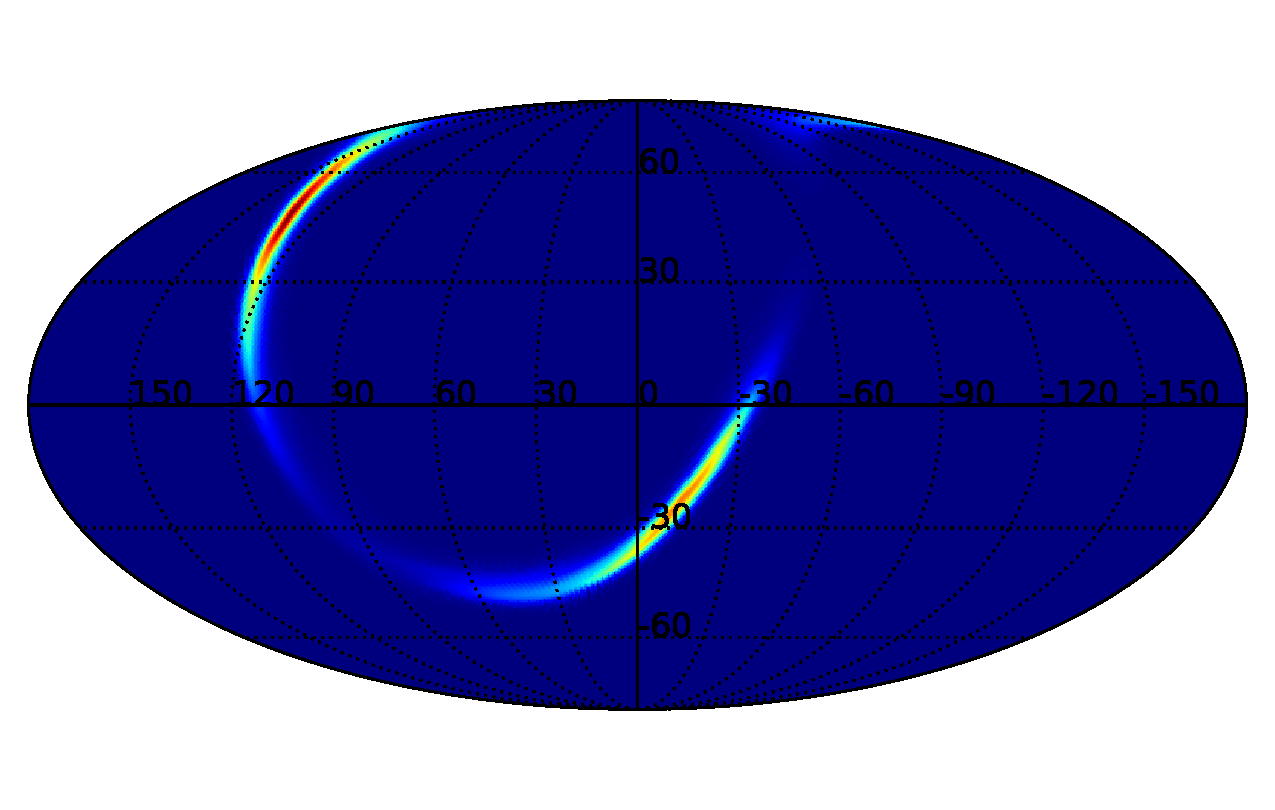
\includegraphics[width=3in]{prob.pdf}
\caption{The gravitational-wave posterior probability distribution $L_\textrm{GW}(\alpha,\delta)$ (marginalized over distance) for GW170104.}
 \label{fig:skymap}
 \end{figure}

\begin{lstlisting}
python gwemopt_run --doEvent --do3D --event G268556
\end{lstlisting}

GraceDB is a service that provides information on candidate gravitational-wave events and the multi-messenger followups performed on them. An API is made available that allows for access to this information.
\emph{gwemopt} uses this API to access information pertinent for gravitational-wave followups.
First of all, it downloads the gravitational-wave skymap for a given event; an example is shown in Figure~\ref{fig:skymap}.
In addition, information such as the time of the event and the time delay between the time-of-arrivals at the detectors is noted.

\subsection{Telescope configuration}
\label{subsection:config}
\begin{lstlisting}
python gwemopt_run --doEvent --do3D --telescope LSST
\end{lstlisting}
\begin{table*}[t]
\scriptsize
\centering
\begin{tabular}{|c|c|c|c|c|c|c|c|c|}
\hline
Telescope & Latitude {[}deg{]} & Longitude {[}deg{]} & Elevation {[}m{]} & FOV {[}deg{]} & FOV shape & Filter & Exp. time {[}s{]} & Lim. Mag. \\ \hline
ATLAS          & 20.7204            & -156.1552           & 3055.0            & 5.46                                      & Square              & c      & 30.0                  & 18.7               \\ \hline
Pan-STARRS     & 20.7204            & -156.1552           & 3055.0            & 1.4                                      & Circle              & i      & 45.0                  & 21.5               \\ \hline
BlackGEM       & -29.2612           & -70.7313            & 2400.0            & 2.85 & Square              & g      & 300.0                 & 23.0               \\ \hline
LSST           & -30.1716           & -70.8009            & 2207.0            & 1.75                                      & Circle              & r      & 30.0                  & 24.4               \\ \hline
ZTF            & 33.3563            & -116.8648           & 1742.0            & 6.86  & Square              & r      & 30.0                  & 20.4               \\ \hline
\end{tabular}
\caption{Configuration of telescopes.}
\label{table:config}
\end{table*}

\emph{gwemopt} relies on standardized configuration files for the telescopes to be analyzed (please see \footnote{https://github.com/mcoughlin/gwemopt/tree/master/config} for examples for the telescopes in Table~\ref{table:config}). 
The information in these files includes the filter being used, the limiting magnitude of the instrument, the exposure time required to achieve that magnitude, site location information, and information about the shape and size of the field of view (FOV). 
Different telescopes have different FOV shapes.
For this, two options, square and circle are available, with the FOV being specified by the length of the square side and the radius of the circle. In addition, a tesselation file, which encodes the placement of the fields on the sky, is requested. This is especially useful for telescopes such as ZTF which use fixed telescope pointings. Fixed telescope pointings can be useful for ensuring the availability of reference images, which are useful when performing image subtraction to look for transients. In case a tesselation file is not available, one is automatically generated, and this output is described in the next section.
Configuration files for ATLAS, BlackGEM, LSST, PS1, and ZTF are available.
Table~\ref{table:config} provides the information assumed for these telescopes.\\

\subsection{Skymap tiling}
\label{subsection:tiling}
\begin{lstlisting}
python gwemopt_run --doEvent --do3D --doTiles --doPlots --tilesType ranked
\end{lstlisting}
Once a telescope configuration has been determined, the next step of the analysis is to generate the sky-map tiling.
There are a variety of algorithms in the literature for sky-map tiling, and the ones implemented in \emph{gwemopt} will be detailed below. The idea is to cover the sky with tiles the size of the telescope's field-of-view with minimal overlap. In some cases, these tiles are pre-determined by survey constraints in order to simplify difference imaging, where a reference image is subtracted from a science image to facilitate transient identification. In other cases, it is possible to optimize the tile locations based on the gravitational-wave skymaps, such that the tiles maximize the probability contained. Due to the FOV for these telescopes being in general much smaller than the probability region, the effect is expected to be relatively minimal.
For example, the number of tiles chosen to allocate time to will be dominated by choices such as whether there is utility in filling in chip gaps (gaps in the CCD arrays that compose the entire camera) and thereby having overlapping tiles, as opposed to simply maximizing the probability contained.
\begin{figure*}[t]
    \centering
    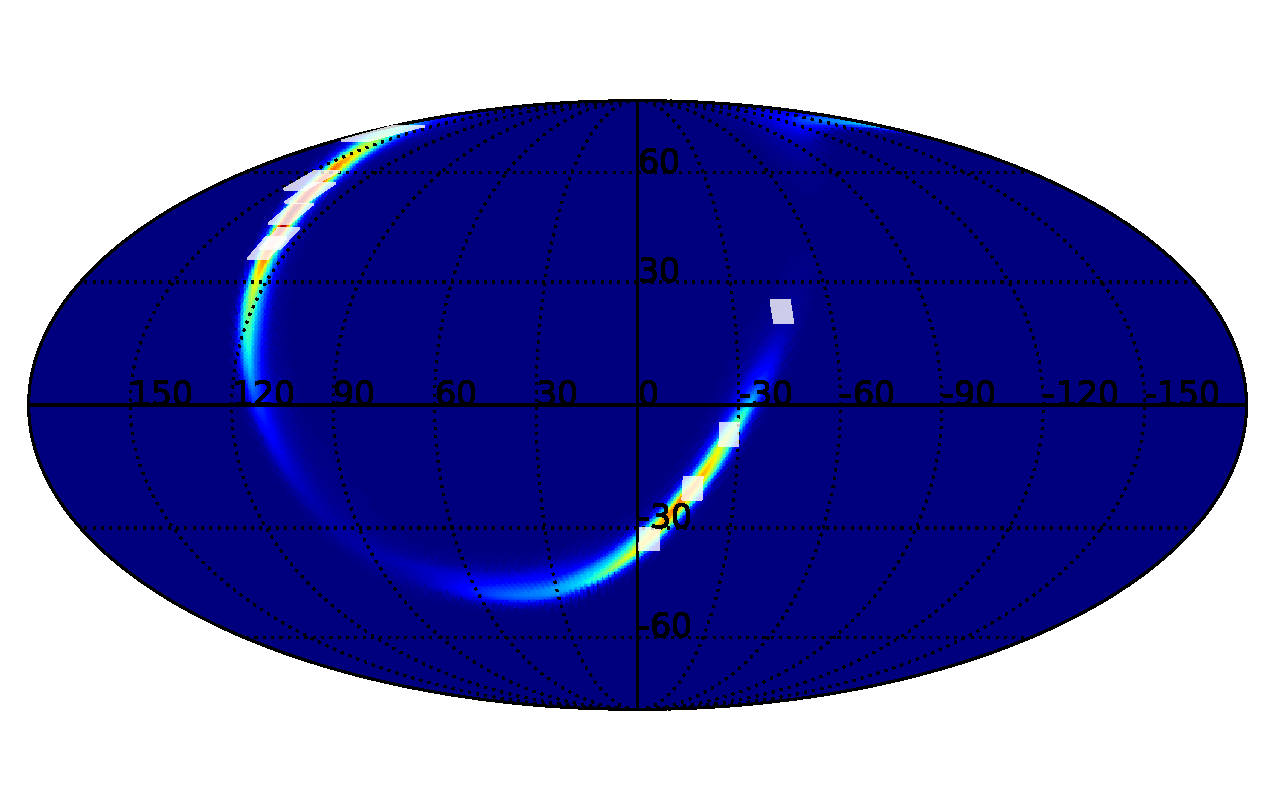
\includegraphics[width=3in]{tiling_greedy}
    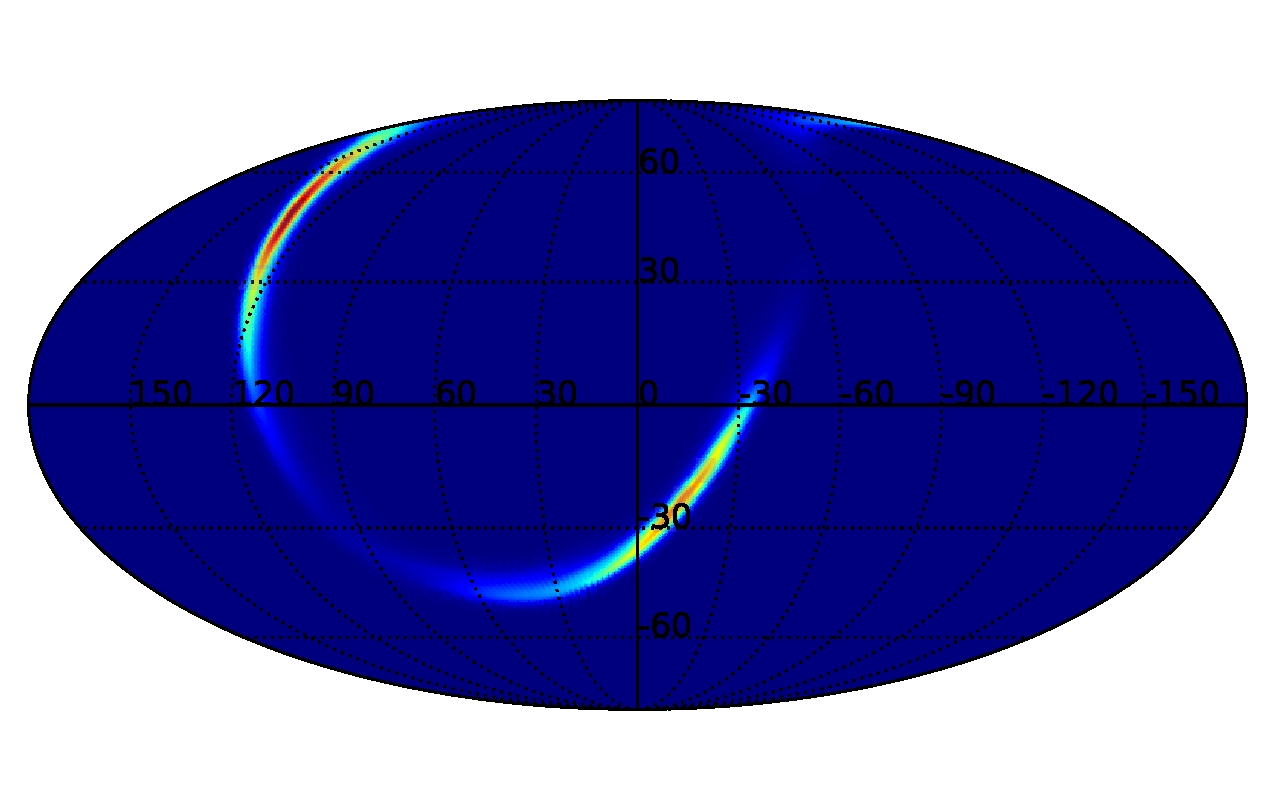
\includegraphics[width=3in]{tiling_hierarchical} \\
    Greedy \hspace{2.6in}Hierarchical\\
    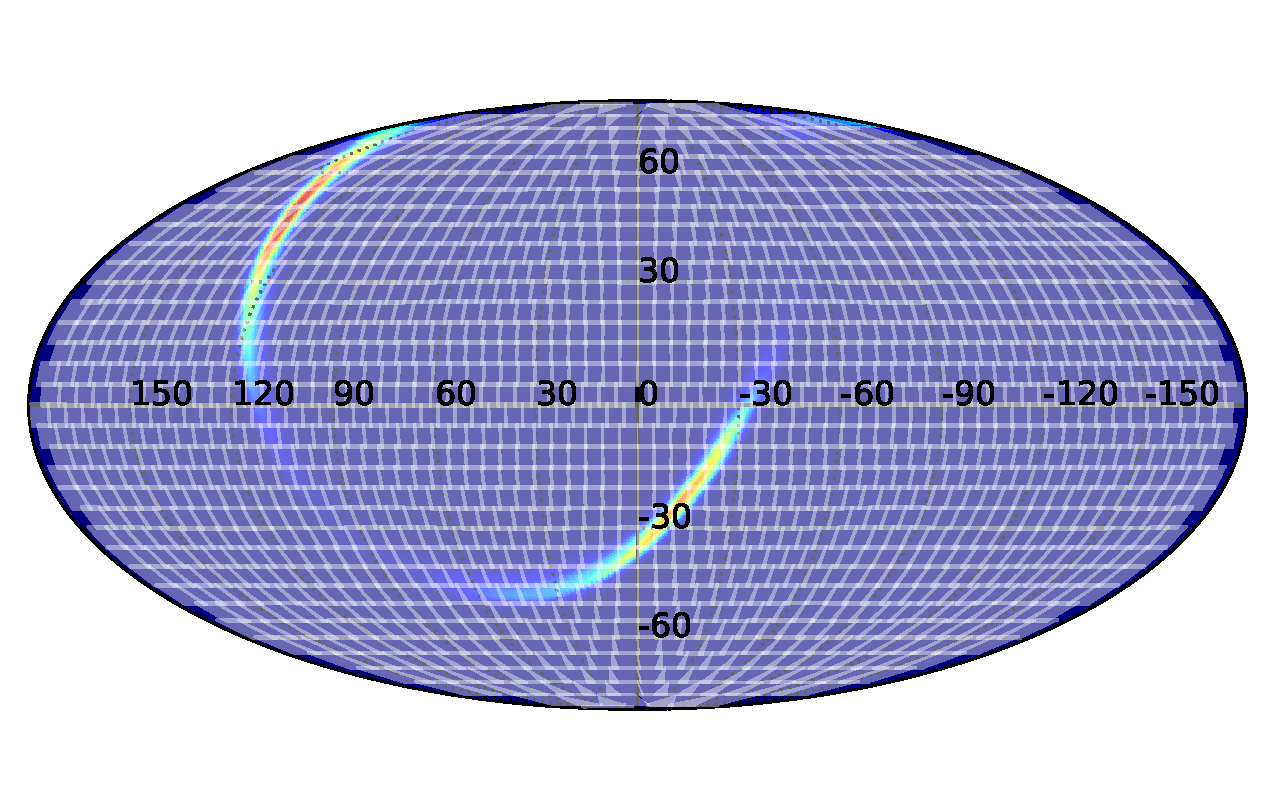
\includegraphics[width=3in]{tiling_moc}
    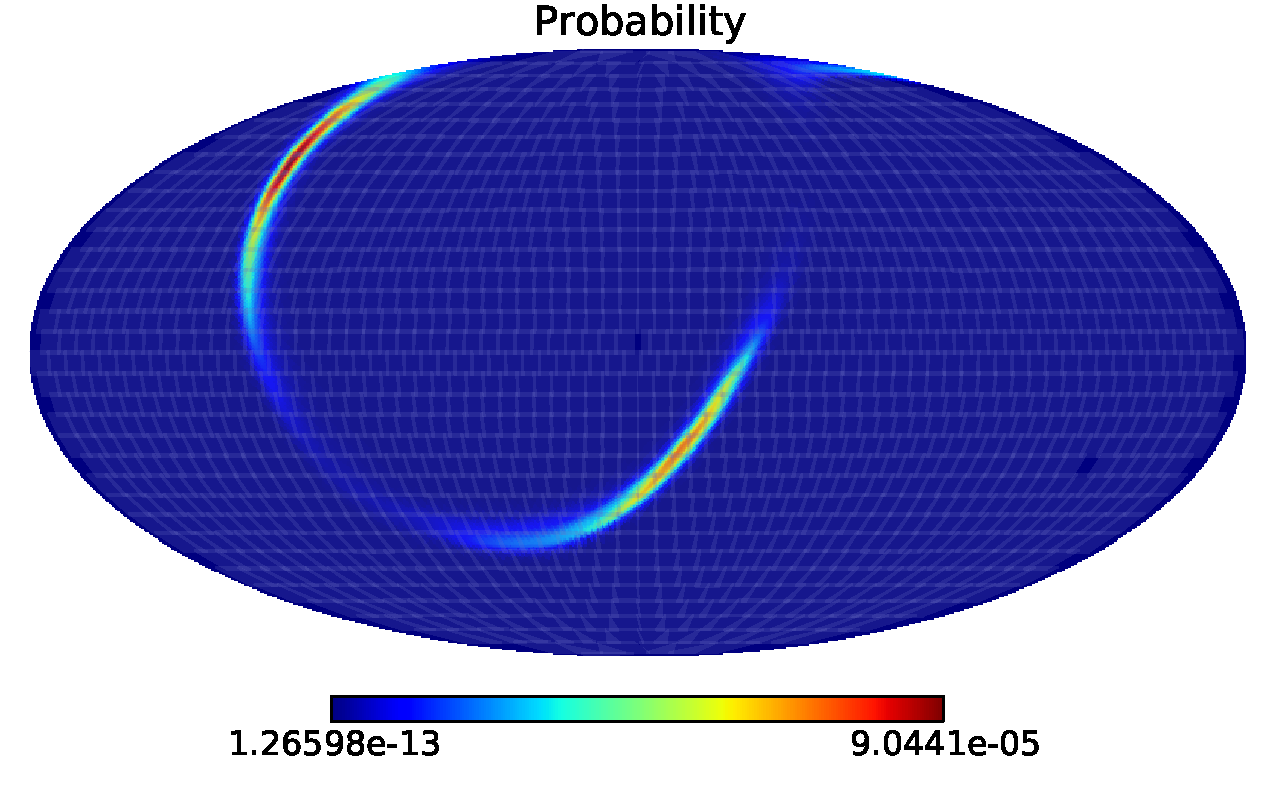
\includegraphics[width=3in]{tiling_ranked} \\
    MOC \hspace{2.6in}Ranked
    \caption{Example outputs of different tiling algorithms. On the top left is the greedy version with $N_{\rm tiles}$ = 10, where $N_{\rm tiles}$ is the number of tiles employed, on the top right is the hierarchical version with the same, on the bottom left is the MOC skymap, and on the bottom right is the ranked skymap tiling. The top row of skymaps are similar, given that 10 tiles are used for both algorithms. The differences between the two schemes, one of which places the tiles all at once and the other places them sequentially, when integrating the probabilities, leads to minor differences in tile placement. The bottom row, with two schemes that cover the entire grid, are identical up to small numerical differences. This is expected as MOC is an on-the-fly scheme, and ranked pre-computes the tile locations.}
    \label{fig:tiling}
\end{figure*}
Gravitational-wave skymaps in general contain metrics that report the spatial probability of a gravitational-wave source lying within a certain location.
They are composed of HEALPix arrays that encode either the 2D probability, in right ascension and declination, or 3D probability, which includes probability distributions for the luminosity distance of the transient.
These are reported in maps with a particular number of pixels, usually $\textrm{N}_\textrm{side} = 512$. 
This can introduce quantization errors, which arise from using a map of limited resolution, especially for small FOV telescopes. 
The --nside flag allows for the up-sampling and down-sampling of the skymaps in the analysis.

There are four options related to skymap tiling currently available and defined below: ranked, MOC (multi-order coverage), hierarchical and greedy.
In the following, we will summarize the key features of each implementation, and refer the reader to the literature for further details.
The goal is to create a common mathematical formalism for straightforward comparisons between algorithms.

\emph{ranked}. The ranked tiling scheme, described in \cite{GhBl2016}, uses pre-defined sky cells (see Fig. 2 of \cite{GhBl2016} for a visualization of how this tiling is performed). This tiling scheme is based on a grid system with grids of equal sizes. The sizes of the grids are the same as the size of the telescope FOV. For each tile in the grid at $(\alpha_i, \delta_i)$, where $\alpha_i$ is the right ascension and $\delta_i$ is the declination, we calculate a double integral that accumulates the probability distribution in this tile, shown in Eq.\ref{eqn:tile_ranked},
\begin{equation}\label{eqn:tile_ranked}
T_{ij} = \int_{\alpha_i}^{\alpha_i+\Delta \alpha}\int_{\delta_i}^{\delta_i+\Delta \delta}L_\textrm{GW}(\alpha,\delta)d\Omega
\end{equation}
where $L_\textrm{GW}(\alpha,\delta)$ is the sky location probability of the event as a function of right ascension and declination, as derived from the analysis of gravitational-wave data.
Then, we rank all the tiles with their $T_{ij}$ and select from the top of the rankings until we reach the target integrated probability desired.
In the following, we will take 95\% as our target integrated probability, which is a reasonable trade-off between capturing as many potential counterparts as possible while also limiting the sky coverage required. Other integrated probabilities could also be considered, and the ideal choice will depend on a trade-off between a few different priorities. These could include the desire to take at least one image of a potential counterpart by covering nearly the entire probability region; another possibility is to take enough images of the same fields to determine the candidates that are appropriately fading and reddening by mapping out their luminosity and color and time evolution.

\emph{MOC}. The ``MOC'' tiling scheme, based on the multi-order coverage of HEALPix maps, hierarchically predefines cells in order to specify arbitrary sky regions \citep{FeBo2014}. 
MOC is proposed in order to provide ``fast set operations'' between regions on the sky, which are designed to minimize computational time for standard set operations (unions, intersections, etc.). In MOC, the spherical sky is recursively divided into 4 regions and each region is a diamond. 
The division stops according to the resolution necessary for a particular usage.
MOC is particularly useful in the case that most information is contained in just a handful of pixels, and therefore it is desired to save that information at high resolution for those pixels, and the remainder of the map at low resolution.
This is important to be both memory efficient and retain all the relevant data.

Here are three relevant implementation details about MOC.
\begin{itemize}
\item MOC uses an equatorial coordinate system. 
\item MOC divides the sphere recursively into four diamonds. 
\item MOC indexes each tile as follows: the initial tile is numbered 0 on level 0. Then, when divided, we get tile indices of 0, 1, 2, 3 on level 1. More generally, if we start from a tile numbered M, its children will be numbered $M\times 4$, $M\times 4 + 1$, $M\times 4 + 2$,$M\times 4 + 3$ on the next level.
\end{itemize}

The scheme for integrating probability in tiles is the same as in ``ranked'' above.

\emph{hierarchical}. The hierarchical tiling scheme, which is a MultiNest-based \citep{FeHo2009,FeGa2009,BuGe2014} optimization, chooses tiles for a given skymap by placing them sequentially on the skymap and maximizing the probability at each step. 
This is distinctive from the ranked scheme in that it does not use pre-defined sky cells.
MultiNest was chosen because with many live points available, multiple live points could simultaneously explore multiple portions of the skymap at once. 
This helps to overcome any potential issues that arise from natural bi-modality of gravitational-wave skymaps, where a single chain could be caught on a single island.
We note that any algorithm designed for high-dimensional sampling is possible here. This method starts by selecting the tile that covers the most probability. Then, it sets the probability in that tile to be zero before going to the next iteration, when it again selects the tile that covers the most probability. The algorithm stops when a user-specified number of tiles, $N_{\rm tiles}$, are selected. The tiles selected might overlap on the corners when there are higher probability distributions around that corner. 
 
\emph{greedy}. The greedy tiling scheme, an emcee \citep{FoHo2013} based algorithm, optimizes tiles for a given skymap by placing all tiles simultaneously on the map. This allows all tile locations to vary at the same time. Similar to the ``hierarchical'' case, any high-dimensional sampler would be reasonable to use here. The algorithm works by taking the user-specified number of tiles, $N_{\rm tiles}$, and allowing the tile locations to vary. It uses a likelihood that maximizes the integrated probability. It prevents double counting by setting the probability of a given tile to zero when integrating the probability. This method selects tiles that cover the highest integrated probability from the skymap. It ranks all possible tiles and selects from the top. Thus, the tiles selected by greedy methods might overlap significantly when the probability distribution is concentrated. 

\subsection{Time allocations}
\label{subsection:timeallocation}
\begin{lstlisting}
python gwemopt_run --doEvent --doPlots --doTiles --doSchedule --timeallocationType coverage
\end{lstlisting}
Having decided on the preferred set of tiles, exposure time allocation forms the next important constraint to
address. 
Because telescopes have fields of view that are in general smaller than the probability region and typical exposure times for these telescopes are of order minutes (see Table~\ref{table:config}), it is, therefore, not possible to image the entire probability region to interesting limiting magnitudes in a reasonable amount of time.
There are further constraints that arise from the diurnal cycle, observing time available for followup, limitations on the pointing that a particular telescope is capable of (such as horizon limits), and the rising and setting of tiles.
The following algorithms use a variety of methods to optimize the probability of imaging a counterpart with the constraint of limited telescope resources.

The amount of time allocated is defined with a few constraints. 
First of all, time segments are generated based on the observing time allocated after the gravitational-wave event. 
In the following analyses, we will assume that 72 hours following the event are available for followup (the code can account for limited target of opportunity time by breaking the time into segments).
The segments are then intersected with night time at the site of the particular telescope, which defines the segments that can be used for observations. 
This assumes implicitly that the electromagnetic counterpart has not faded beyond detection limits in the time available. 
Some of the time allocation algorithms below use models to determine the detectability of the lightcurve.
There are four options related to time allocations as a function of sky location, coverage, powerlaw, WAW (Where and when), PEM (Probability of electomagnetic counterpart). Figure~\ref{fig:timealloc} shows examples of the powerlaw, WAW, and PEM types.

\emph{Coverage.} The ``coverage'' option is one whereby coverage from existing surveys, including the right ascension and declination of the pointing and the limiting magnitude, are used. The benefit of this mode is to establish efficiencies of detection of kilonovae in existing surveys. For example, this code will be used to determine the efficiencies of the Pan-STARRS and ATLAS surveys to both gravitational-wave and gamma-ray burst triggers. It can be used as a way to prioritize examination of survey data for serendipitous observations of these transients, where both reference images and the time of the transients are known.

\emph{Powerlaw.} The ``powerlaw'' option is one where scaling relations are applied to the probability map to determine the time allocation.
Many authors \citep{GhBl2016,CoSt2016a,ChHu2017} have proposed a variation on simply scaling the time allocation proportional to the probability skymaps, a technique employed in the powerlaw method below.
Pan-STARRS and ATLAS based searches have employed this technique \citep{SmCh2016,SmCh2016b,StTo2017}.
\cite{CoSt2016a} derived scaling relations for the time allocated to any given field, $t_i$, given the gravitational-wave posterior probability distribution. While the powerlaw based analysis is straightforward, it does not account for the fact that the telescope must be sensitive enough to detect the counterpart. In this sense, this algorithm is the least model dependent. The detectability of a given transient is model-dependent, depending both on the distances predicted by the gravitational-wave data analysis and the absolute magnitude of the sources; the following algorithms account for this dependnce in multiple ways.

The \emph{Powerlaw} algorithm optimizes the probability of detecting the transient with N observations, which is simply the sum of the probability of each observation. The expression is shown in Eq.\ref{eqn:powerlaw}:
\begin{equation}\label{eqn:powerlaw}
p_{tot}=\Sigma_{i=1}^N \frac{M_i}{M_{tot}}\frac{L_{GW}(\alpha_i, \delta_i, R_i)}{L_{GW_tot}}\frac{F_i(t_i)}{a(\alpha_i, \delta_i)},
\end{equation}
where $R_i$ is the distance to the galaxy, $M_i$ is the mass for galaxy $i$, $M_{tot}$ is the total mass of galaxies in the field, $L_{GW}(\alpha_i, \delta_i, R_i)$ is the posterior probability distribution of the gravitational wave source in this galaxy, $F(t)$ is the luminosity as a function of allocated time, and $a(\alpha_i, \delta_i)$ is the Galactic extinction. In the following, we will simply scale the gravitational-wave posterior probability distribution as $L_\textrm{GW}(\alpha_i,\delta_i)^{2/3}$ (as shown by the analysis of \cite{CoSt2016a} to be optimal given their assumptions). Within this formalism, independent scaling of the distance is also possible (such as with $R^4$ to maintain a constant electromagnetic signal-to-noise ratio for a particular target absolute magnitude) , but this dependence has been accounted for in calculating the sky map probability's associated powerlaw. It is possible that this approximation could be improved using galaxy catalogs, although this introduces concerns about galaxy catalog completeness. Eq.~\ref{eqn:powerlaw} is optimized with the constraint that the total observation time is limited, shown as
\begin{equation}
\Sigma_{i=1}^N t_i=T,
\end{equation}
where $T$ is the total observation time.

\emph{WAW.} The ``When and Where'' algorithm, defined in \cite{SoCo2017}, uses counterpart lightcurve models in the optical, infrared and radio constructed from information from the gravitational-wave signals to create a time- and sky location dependent probability for detecting electromagnetic transients. The WAW approach introduces time into the model by defining a concept of detectability. Detectability is the probability of detecting a light flux greater than the flux limit at position $\alpha$ and time $t$. These flux limits are computed using a combination of lightcurve models and knowledge of distance to the counterparts for compact binary coalescences. Thus, by having detectability introduced, the algorithm can optimize "where" and "when" to schedule the observation based on $\alpha$ and $t$ with a greedy approach. The procedures of the algorithm are shown below.
\begin{enumerate}
\item The tiles are generated covering the confidence region based on the probability distribution, which comes from the gravitational wave signal.
\item The algorithm takes in the information encoded in the gravitational waves and computes the lightcurve $F_i(t)$ for each tile. 
\item Then, the algorithm computes the detectability as
\begin{equation}\label{eqn:detectability}
P(F(t) > F_{lim}|\alpha, S)\approx\Sigma_{i=1}^N\omega_i H(F_i(t)-F_{lim})
\end{equation}
where $H$ is the Heaviside function where if $F_i(t)$ is greater than $F_{lim}$, it is 1; otherwise it is 0. $F_i(t)$ is the light flux for position sample $i$ at time t. $F_{lim}$ is the limiting flux, which is the minimum detectable flux by the instrument. $\omega_i$ is the "inverse distance weight" that gives the contribution of the sample $i$ to position $\alpha$. The further away sample $i$ is from $\alpha$, the less it contributes. $\omega_i$ is normalized so that $\Sigma_{i=1}^N\omega_i=1$. 
\item For each tile, we find a time interval $[t_{E,\lambda},t_{L,\lambda}]$ when the detectability is greater than a threshold $\lambda$.
\item We start from the tiles that cover the most probability and arrange their observation times $[t_{E,\lambda},t_{L,\lambda}]$ if the time is available.
\end{enumerate}
This method optimizes the search by introducing detectability, defined as Eq.~\ref{eqn:detectability} over the three dimensional observation volume of direction and time, with the constraint that only one location can be observed at the same time.

\emph{PEM.} The ``Probability of electromagnetic counterpart'' algorithm, defined in \cite{ChHu2017}, optimizes the number of fields to observe and their time allocations by adopting priors on the intrinsic luminosities of the sources and using knowledge of distance to the counterparts for compact binary coalescences. More concretely, its input is the sky localization map and information about the telescope. It selects the tiles to observe with a greedy algorithm and allocates the observation time for each tile to maximize the probability of detecting the EM counterpart of the GW event. 

The procedures of the algorithm are shown below, and further details can be found in \cite{ChHu2017}.
\begin{enumerate}
\item Based on the sky localization map, we locate the tiles that cover the region enclosed by the contour of the target confidence level.
\item These N tiles are ranked based on the total probability covered.
\item We optimize the number of tiles selected and then the time allocation for each selected tile. For all $k$ from 1 to n, we do the following:
\begin{itemize}
\item the top $k$ tiles from the rankings are selected. 

\item Eq.~\ref{eqn:pem_obj} is the total detection probability of all the tiles and optimized with Lagrange multipliers with the constraint of Eq.~\ref{eqn:pem_const}, which encodes the limited observational time on the telescope: 
\begin{equation}\label{eqn:pem_obj}
P(D_{EM}|k)=\Sigma_{i=1}^{k\leq n}P(D_{EM}|\omega_i^{(k)}, \tau_i^{(i)},I)
\end{equation}
\begin{equation}\label{eqn:pem_const}
k T_0+\Sigma_{i=1}^k\tau_i^{(i)}=T
\end{equation}
where $\omega_i$ is the probability density; $\tau_i$ is the time allocated and $I$ are the parameters of the telescope, $T_0$ is the time to adjust the telescope before each observation, $\tau_i$ is the time allocated to each tile, and $T$ is the total observation time.
\item Eq.~\ref{eqn:pem_obj} is maximized with the constraint of Eq.~\ref{eqn:pem_const} to determine the best $k$, the tiles and the time allocation.
\end{itemize}

\item The optimal tiles $\{\omega_i\}$ and their allocated times $\{\tau_i\}$ for $i=1...k$ are the output.
\end{enumerate}

\begin{figure*}
    \centering
    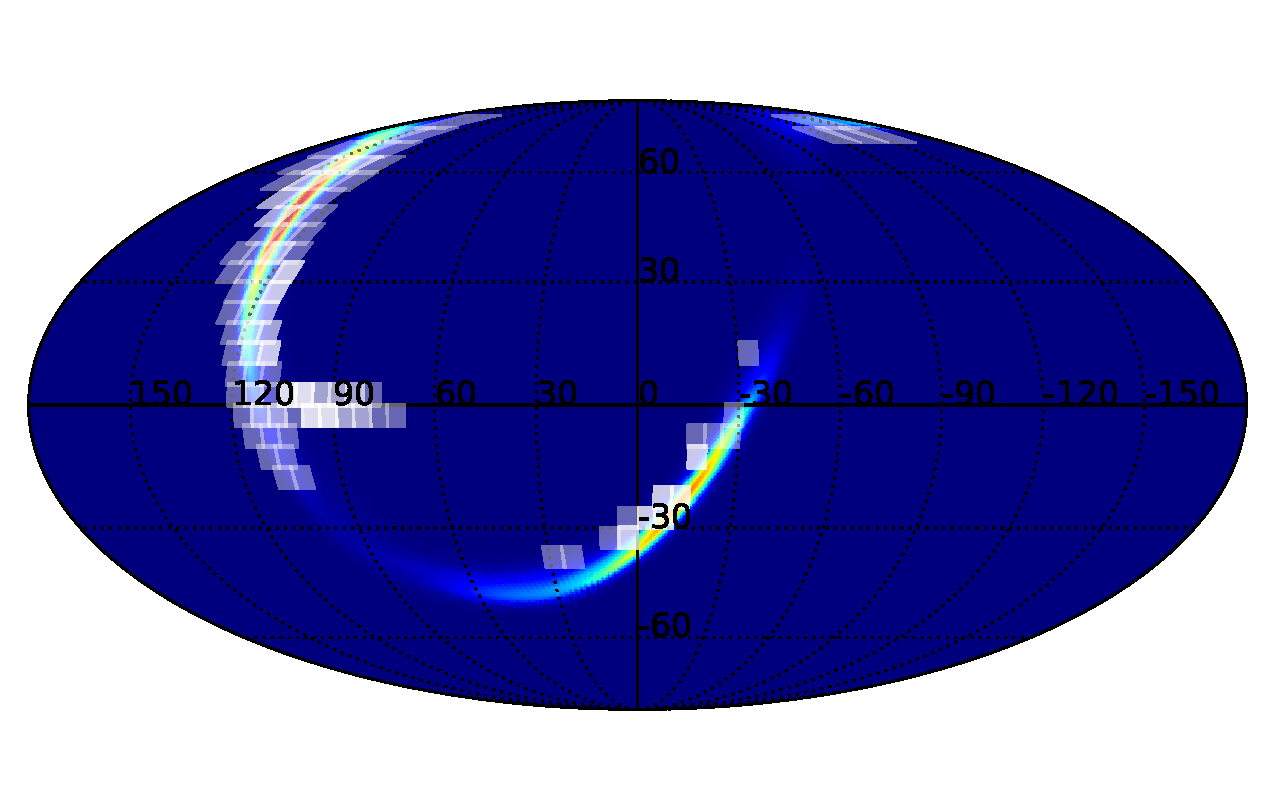
\includegraphics[width=3in]{plots/coverage_pem.pdf}
    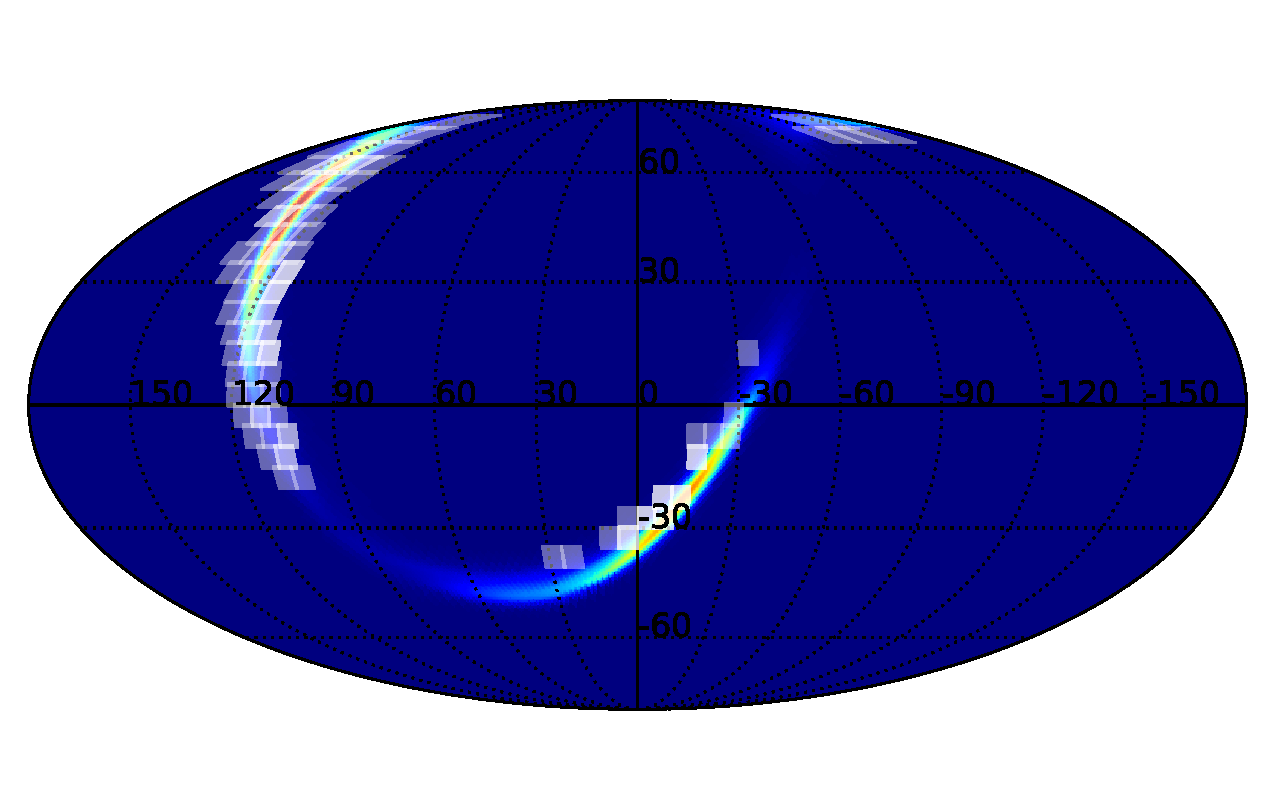
\includegraphics[width=3in]{plots/coverage_powerlaw.pdf}\\
    PEM\hspace{2.6in}Powerlaw\\
    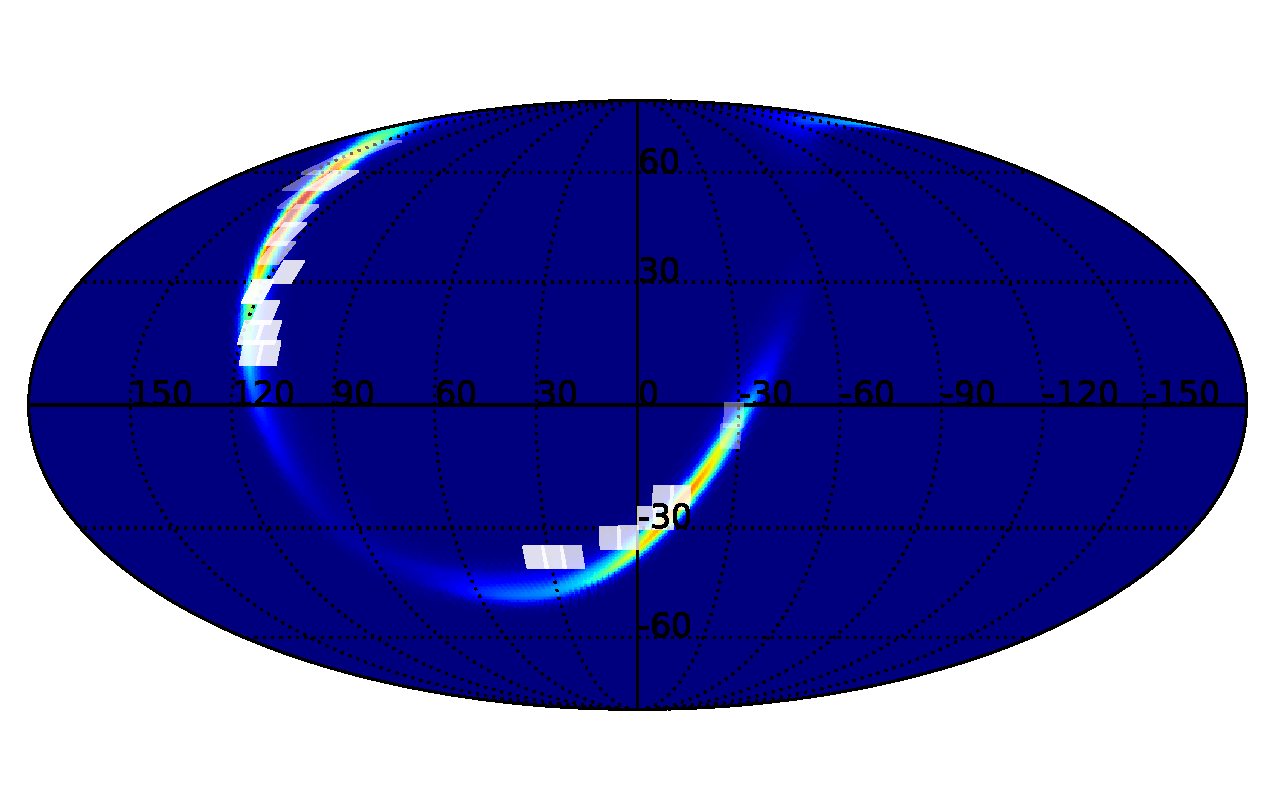
\includegraphics[width=3in]{plots/coverage_waw.pdf}\\
    WAW
    \caption{Example outputs of different time allocation algorithms. On the top left is the tile coverage with the PEM algorithm. On the top right is the tile coverage with the Powerlaw algorithm. On the bottom is the tile coverage with the WAW algorithm. In generating all of the plots, the MOC algorithm is used. Given the differences in the algorithms discussed in the text, it is unsurprising that some differences in the time allocations are seen.}
    \label{fig:timealloc}
\end{figure*}


\subsection{Scheduling}
\label{subsection:scheduling}
\begin{lstlisting}
python gwemopt_run --doEvent --doPlots --doTiles --doSchedule --scheduleType weighted
\end{lstlisting}
Once the time allocated to each tile has been set, the next task is to schedule the observations that both best represent the time requested and optimize the times that are chosen in some way. 
For example, the tiles could be re-imaged at an approximately fixed cadence so as to measure possible lightcurve evolution.
Another option is to simply go as deep as possible in one field to ensure detection of a counterpart there.
Other optimizations might employ ordering based on airmass (or the amount of atmosphere a telescope observes through), as sources imaged through higher airmass will have lower signal-to-noise ratios.

For each of the algorithms that perform the scheduling, the time that each tile is available for observation above the altitude limit, which corresponds to the lowest altitude a telescope can observe (assumed to be $30^\circ$ in this analysis), is computed.
These tile-specific times are intersected with the set of times available to the telescopes to form a set of visibility segments for each tile.
This has the benefit of avoiding issues related to simply tracking the rise and set times of each tile.
To account for lunar sky brightness, we use a model from \cite{CoSt2016b}. 
Any tile whose sky brightness is increased by at least 1\,mag is excluded.

There are three options related to scheduling observations: greedy, sear, and weighted.
\emph{Greedy.} The ``greedy'' algorithm, which is the simplest version in the code package, employs a schedule on the basis of probability contained. The idea is that higher ranked tiles are observed before lower ranked tiles based on this ranking scheme. \cite{RaSi2017} implements a greedy algorithm whereby the field with the highest probability region in a given time window is observed. As the \cite{RaSi2017} implementation does not include the possibility of multiple exposures for each pointing, it is modified in this analysis to include multiple exposures. The algorithm is as follows:

\begin{enumerate}
\item Construct a list of the tiles and number of exposures for each tile based on the time allocation algorithm utilized.
\item For each window, find the sky tiles that are in the current window: $T_0 + (j-1) T_{exp}$ and $T_0 + j T_{exp}$, where $T_0$ is the start time for the observation, $T_{exp}$ is the exposure time, and $j$ is the index of the window.
\item Allocate the window to the sky tile with the greatest probability, and increment the number of exposures for that tile down by 1.
\end{enumerate}

\emph{sear (Setting Array).} The ``Setting Array'' algorithm, overcomes the shortcoming of the greedy algorithm to include site visibility. This motivates re-ordering the sequence such that as many tiles can be imaged as possible.
\cite{RaSi2017} also implements a version whereby the rising and setting of tiles were accounted for. Sear prioritizes observing high probability tiles first, subject to the condition that each tile from the observing sequence must be observed before it sets. The concept of imaging ``windows'' are used in this algorithm, where the available observational time is broken up into segments referred to as windows. We denote the $i$th window as $W_i$. We denote the tile that will be imaged in window $W_i$ as the tile $S_i$. The algorithm uses the recursive relation between the optimal observation arrangement between the first $k$ windows {$S_1$ ... $S_k$} and the $k + 1$ window $S_{k+1}$. The details are shown below. 
\begin{enumerate}
\item Consider the first window $W_1$ and initialize $S_1$ to be the tile that has the highest probability for $W_1$.
\item Move on to $W_2$ and find the two tiles $c_1$ and $c_2$ that have the greatest probability density.
\item Compare $c_1$ and $c_2$ with $S_1$ and act depending on the following conditions:
\begin{itemize}
\item If both $c_1$ and $c_2$ contain greater probability than $S_1$, set $S_1$ = {$c_1$} and $S_2$ = {$c_2$}.
\item Otherwise, put the tile with higher probability coverage between $c_1$ and $c_2$ into $S_2$; $c_2$ is then assigned to $S_3$.
\end{itemize}
We can see that either way, $S_1$ and $S_2$ will have the two highest probability tiles observable.
\item Move on to the next observation window and repeat until the last one is reached.
\item Return the last set $S_w$ where $w$ is the total number of observation windows.
\end{enumerate}

\emph{weighted.} A different scheme, known as ``weighted,'' is an algorithm where each tile is weighted based on both gravitational-wave posterior probability distribution enclosed, the number of exposures required for that tile, and the number of available slots for it to be imaged. This is an alternative to greedy and sear, as it is impossible to observe all of the tiles as they rise and set given the requirement of using multiple exposures per tile. 

The idea is that all of the tiles are given a weight that depends on the requested number of exposures. 
Therefore we define the weights $w_i$ as
\begin{equation}
w_i = L_\textrm{GW}(\alpha_i,\delta_i) \times \frac{N_\textrm{R}}{N_\textrm{A}} 
\end{equation}
where $N_\textrm{R}$ is the number of remaining images to be taken for a given tile and $N_\textrm{A}$ is the number of allocated exposures for that tile.
In this way, $\frac{N_\textrm{R}}{N_\textrm{A}}$ prioritizes the tiles with the most remaining exposures.
Therefore, for each exposure segment, we calculate the weight for each possible tile and select the tile with the highest weight to fill that slot.
\subsection{Efficiency}
\label{subsection:efficiency}
\begin{lstlisting}
python gwemopt_run --doEvent --doPlots --doTiles --doSchedule --doEfficiency
\end{lstlisting}
We are able to test and compare the performance of these algorithms by performing simulated observations. 
We adopt observational constraints as follows. 
We use an observing limit of an altitude of 30$^\circ$, corresponding to an airmass of 2.0. 
We assume observations are available to begin at twilight and dawn, corresponding to when the sun is 12$^\circ$ below the western and eastern horizons.
We do not point away from the moon or account for sky brightness.

The simplest metric of success is the ``efficiency,'' which is defined as the number of transients detected over the number of transients injected.
To estimate the efficiency for the ``detection'' of the electromagnetic counterparts to gravitational-wave transients, we perform simulated injections of supplied lightcurves, which corresponds to the absolute magnitude in the color requested in the telescope configuration file. 
The number of transients injected are proportional to the values in the sky localization probability map to account for the selection effects of the gravitational-wave detector network.
We provide example lightcurves for a variety of lightcurve models, including:

\begin{enumerate}
\item \cite{TaHo2014}: Simulations of binary systems showing ejecta morphology and resulting lightcurves. These simulations led to analytical models for black-hole neutron star systems from \cite{KaKy2016} and\cite{DiUj2017}.
\item \cite{KaKy2016}: Analytical models for black-hole neutron star systems based on \cite{TaHo2014}.
\item \cite{DiUj2017}: Analog to \cite{KaKy2016} for binary neutron star systems.
\item \cite{BaKa2016}: Simulations of binary systems studying the emission profiles of radioactive decay products from the merger.
\item \cite{MeBa2015}: Blue ``precursor'' to the kilonova driven by $\beta$-decay of the ejecta mass.
\item \cite{Me2017}: Toy model with grey opacity for lanthanide-free matter expanding with a range of velocities with a mass density profile $M(< v) = v^{-1}$.
\end{enumerate}

The requirements for ``detection'' of the electromagnetic counterparts to gravitational-wave transients are as follows.
We require that the transient appear in 2 images over 2 nights.
In each image, the transient must exceed the limiting magnitude in that image.
The color of the transient is estimated from the filter given in the configuration file.
We simulate the transients at a variety of locations and distances consistent with the gravitational-wave probability skymap.


\section{Performance}
\label{sec:performance}
In this section, we compare the efficiency of the algorithms based on simulated information about what percentage of the events the algorithm can detect. According to the workflow given in Figure~\ref{fig:flowchart} and the algorithms given in the sections above, we will have four options for tiling algorithms, three options for time allocation algorithms and another three options for scheduling algorithms. This combines to 36 total options for the whole workflow. We want to know which combination has the best efficiency and then analyze and compare the algorithms individually.
We take as an example the ATLAS instrument in the following. 
As all of the instruments are large aperture, wide-field instruments, the results will not strongly depend on the instrument chosen and the way the efficiencies scale will be the same for the level of detail considered here.
Including information such as slew and readout time of the individual telescopes will change the results in case of lengthy readout times or characteristically slow slew times.
For telescopes with either readout or slew times on the order of the typical length of exposures, the efficiencies could be impacted by up to a factor of 2.
For the survey telescopes we consider in this analysis, they are designed to have short readout and slew times so as to minimize this overhead, and so the loss in efficiency will be much smaller.
\subsection{Method}
We will focus on the model by \cite{Me2017} to compare the efficiency. All the efficiency values in the (logarithmically spaced) distance range between $10^{-1} Mpc$ to $10^3 Mpc$ are calculated and plotted. Thus we will have a plot of efficiency versus distance for each of the 36 algorithm combinations. An example efficiency plot is shown in Figure~\ref{fig:eff_ex}, where different time allocation algorithms are compared. The greedy algorithm is used for tiling and the PEM algorithm is used for time allocation. It can be seen that greedy and sear scheduling does better than weighted for long distances. 

\begin{figure}[t]
\centering
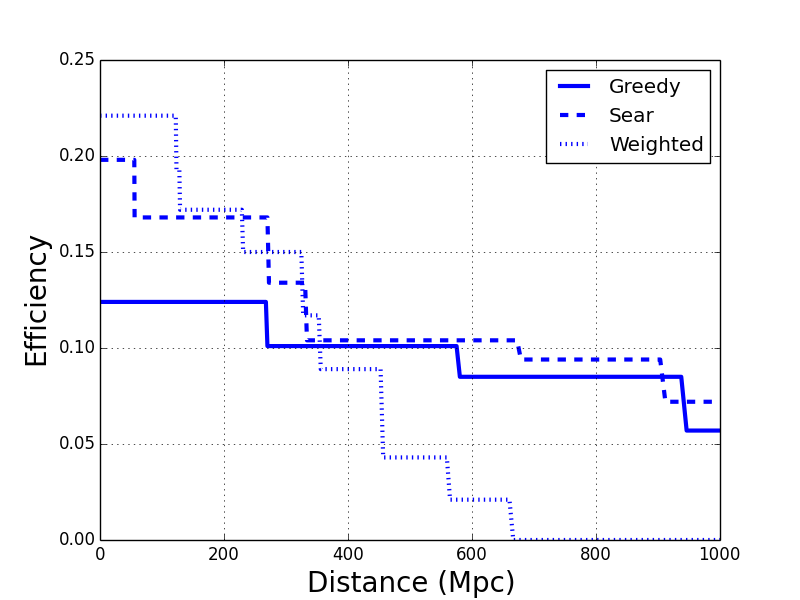
\includegraphics[width=0.5\textwidth]{plots/eff_ex.png}
\caption{Example plot of efficiency for \cite{Me2017} injections, comparing the scheduling algorithms. The constraint for each algorithm was on the total observing time available. The greedy algorithm is used for the tiling and PEM algorithm is used for time allocation. The greedy and the sear algorithms have similar performance for long distances and both perform better than weighted. This difference is also reflected in Figure~\ref{fig:eff_metric}. As the algorithm accounts for observability from a site, including both whether tiles are visible from the site of interest as well as diurnal effects, efficiencies are expected to peak at around 25\% for an event which fades quickly and has a probability region with peaks in both the north and south.}
\label{fig:eff_ex}
\end{figure}
In Figure~\ref{fig:eff_ex}, we show an example where we hold the tiling and time allocation algorithms fixed (to disentangle their effects from the scheduling algorithm), and show the efficiency as a function of distance for the scheduling algorithms discussed in this paper. We find that both Greedy and SEAR perform better than weighted at larger distances. Weighted performs best at the lowest distances considered because it targets the highest probability tiles, ensuring that they will be scheduled for multiple exposures so as to meet the detection criteria. Greedy and SEAR, both of which schedule tiles to maximize the number of fields imaged, with SEAR accounting for the rising and setting of the tiles, perform significantly better at greater distances. This is because they sacrifice some efficiency for nearby sources by effectively exploring more fields, but have a more constant detection efficiency with distance.

In order to compare the 36 efficiencies as plotted in Figure~\ref{fig:eff_ex}, we use a single statistic to reflect the overall performance of the algorithms based on the efficiency for each distance in the range of $10^{-1} Mpc$ to $10^3 Mpc$. Thus, we come to a metric that reflects what percentage of events that can be detected in a spherical volume of radius $10^3 Mpc$. The events are evenly distributed in the volume. Suppose the event density per volume is $\rho$ and the distance is $r$. Sampling a distance at $r$ corresponds to a shell with volume $4 \pi r^2 dr$. Assuming that the density is $\rho$, then the total events on that shell are $4 \pi \rho r^2 dr$. Thus, if the efficiency is $e$, the expected number of detected events on the shell will be $4 \pi \rho r^2 e dr$. From this we can see that the efficiency at $r$ is weighted by $r^2$. If we treat the efficiency at each distance as an individual sample, a weighted average on the squared radius will then be a good metric of the overall efficiency; it reflects how well the algorithm detects events uniformly distributed in a spherical volume of radius $10^3 Mpc$. A consequence of this metric is that the weight of $r^2$ makes the long range efficiency more important than the short range efficiency. Under this metric, an algorithm that performs well at further distances would be better than an algorithm that does better at short distances but whose performance deteriorates quickly as the distance increases. 

\subsection{Performance and algorithms}
\begin{figure}[t]
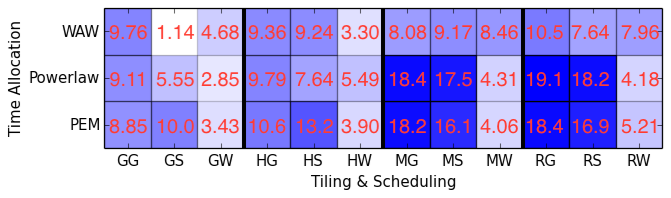
\includegraphics[width=0.45\textwidth]{plots/efficiency.png}
\caption{Plot of the weighted efficiency metric for each of the 36 options. On the horizontal axis are tiling algorithms and scheduling algorithms and on the vertical axis are the time allocation algorithms. Abbreviations are used for the algorithms. The first capital letter stands for the tiling algorithm and the second letter stands for the scheduling algorithm. The abbreviations are the first letters of the algorithms: G - greedy. H - hierarchical. M - MOC. R - ranked. S - SEAR. W - weighted. The grids are colors such that highest efficiency combinations are darker and lower efficiency ones are lighter, with the highest being completely blue and the lowest one being completely white.}
\label{fig:eff_metric}
\centering
\end{figure}
For each of the 36 algorithm options, we compute the efficiency metric as described above, which results in 36 numerical efficiency values. The results are plotted in Figure~\ref{fig:eff_metric}. On the horizontal axis are the combined options for the tiling algorithm and scheduling algorithm. There are four tiling algorithms and three scheduling algorithm so they combine to 12 columns on the horizontal axis. Abbreviations are used for the algorithms. The first capital letter stands for the tiling algorithm and the second letter stands for the scheduling algorithm. On the vertical axis are the time allocation algorithms. The color in the 36 boxes shows the efficiency as measured above. The colors are scaled to the efficiency such that higher efficiencies are more darkly colored.
The highest efficiency of $0.19$ is achieved by a combination of ranked tiling, powerlaw time allocation and greedy scheduling. Compared to the lowest efficiency of $0.01$, it can detect approximately 19 times more events within a range of $10^{-1} Mpc$ and $10^3 Mpc$. That corresponds to the darkest box in the 10th column and the second row in Figure~\ref{fig:eff_metric}. 

Also, from Figure~\ref{fig:eff_metric}, we can compare the efficiencies of the individual algorithms.
We concentrate on the SEAR scheduling algorithm in the following. For example, in the case of the use of the MOC tiling algorithm, where all (non-overlapping) tiles are available for allocation, we can look at the ``MS'' column. The performance of PEM and power-law are very similar, and this fact holds true for all of the configurations. This similarity may be surprising, given that the powerlaw algorithm does not use the distance posteriors like PEM does. Instead, the powerlaw algorithm encodes the way the probability should be allocated with distance in its powerlaw term, and when considering distances where the ``shot-noise'' of galaxies disappears, they become equivalent. WAW suffers somewhat from the lack of the asset that makes it most valuable: inclusion of the dependence of lightcurves on the inclination angle of the original binary. Therefore, it is not surprising that PEM outperforms WAW in this instance, as PEM is optimal in the presence of distance information, while WAW requires inclination information in order to be optimal. However, in case inclination and distance were available in low latency, WAW may be best.
The lower efficiencies in the case of overlapping tiles of the greedy and hierarchical tiling algorithms are due to the upperlimit of the number of tiles posed (to be returned to in the next section), while performing similarly to one another. This is unsurprising, as both algorithms differ only in the order in which tiles are determined (greedy optimizes the location all at once, while hierarchical places one tile after the other).

\subsection{Performance and the number of tiles}

We also study how the number of tiles affects the performance. This study in particular will depend on the FOV of the instrument in question. It is only relevant in the hierarchical and greedy tiling algorithm. The hierarchical algorithm is used for this study, which selects tiles that cover the highest probability and masks the tiles once they are selected. It stops when a user-defined number of tiles is selected. The efficiency is computed based on the simulation of 5000 injections.

From the plot on the left of Figure~\ref{fig:eff_ntiles}, it can be seen that efficiency increases at first when we increase the number of tiles but after a peak is seen around 35 tiles, the efficiency starts decreasing. The right plot shows the efficiency curves for different number of tiles. Red indicates high efficiency; blue indicates low efficiency. It can be seen from the plot that efficiency at the smallest distances continues to improve as the number of tiles is increased. However, as the number of tiles increase, the efficiency for distant sources first rises and then falls (starting around 35 tiles). This occurs because as more tiles are chosen, less overall time can be allocated to the sources which would otherwise require longer exposure times. The most distant sources are found when using approximately 35 tiles and this corresponds to the peak we see in the left figure.
It is important to note that just because a tile is selected by the tiling algorithm, it is not assured that time will be allocated to that tile or it will be scheduled.
It is also important to note that the algorithms presented here do not account for readout or slew times, which will have some effect on these results. For an alternative study that accounts for these effects, please see \cite{ChHu2017}.
\begin{figure*}[t]
    \centering
    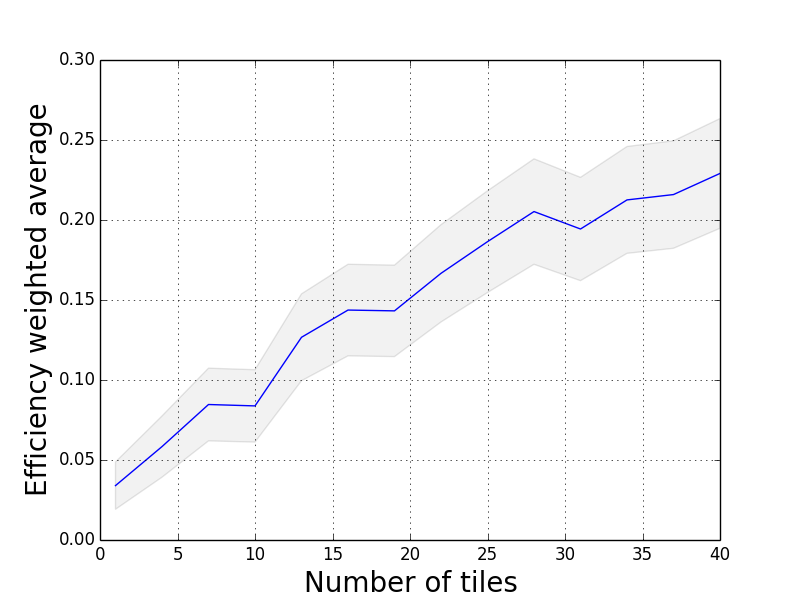
\includegraphics[width=0.45\textwidth]{plots/eff_ntiles.png}
    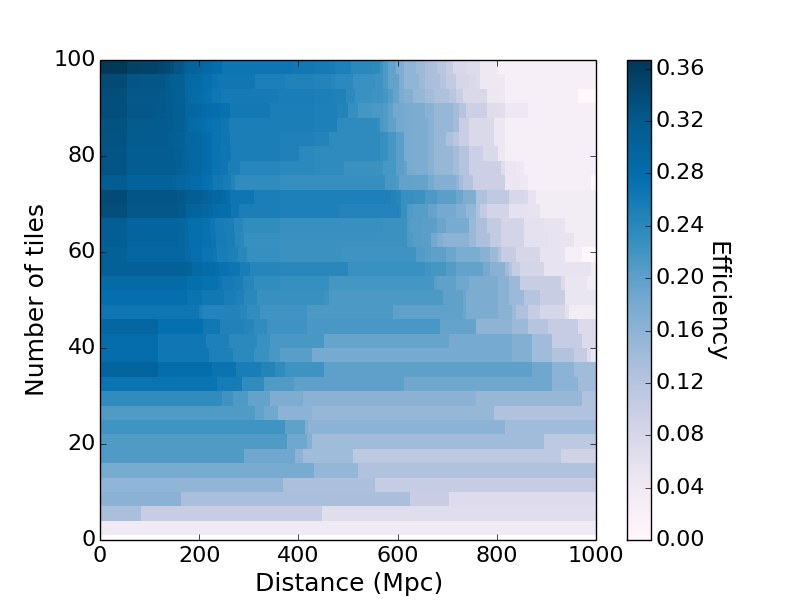
\includegraphics[width=0.45\textwidth]{plots/eff_pcolor.png}
    \caption{On the left is the plot of efficiency weighted average as a function of the number of tiles considered. On the right is efficiency as a function of distance for different number of tiles. In the simulation, hierarchical tiling algorithm, powerlaw time allocation algorithm and greedy scheduling algorithm are used to detect 5000 random injections for number of tiles ranging from 1 to 100. The standard deviation is calculated and the 99\% confidence interval is plotted as the grey shaded region in the top figure. Blue indicates lower efficiency and red indicates higher efficiency. We can see that as the number of tiles increases, low distance gets better but high distance gets worse. We see the least blue at high distance around 35 tiles, which corresponds to the peak in the left plot.}
    \label{fig:eff_ntiles}
\end{figure*}

\section{Conclusion}
\label{sec:conclusions}

The detection of GW170817 \citep{AbEA2017b} has invigorated the search for improved strategies for associating gravitational waves with electromagnetic
counterparts.
Due to the large uncertainty footprint, which can range from 10-1000 square degrees \citep{AbEA2016h}, efficiently scanning sky areas  of this size in search of an electromagnetic counterpart is challenging.
However, in this paper, we have described and compared a number of algorithms in the literature available for significantly improving upon the most naive approaches.
We have shown comparisons between the algorithms, describing the limits in which they are the most effective.

One potential improvement to the analysis considered here is using the locations of known galaxies in the gravitational-wave sensitivity distance, which was $\approx 100$\,Mpc for GW170817 \citep{AbEA2017b} and will extend to $\approx 300$\,Mpc at design sensitivity \citep{AbEA2016h}. 
Recent improvements in galaxy catalog completeness have made this effort possible. For example, the Galaxy List for the Advanced Detector Era (GLADE) galaxy catalog is complete (with respect to a Schechter function) out to $\approx 300$\,Mpc for galaxies brighter than the median Schechter function galaxy luminosity \footnote{http://aquarius.elte.hu/glade/}. The Census of the Local Universe (CLU) catalog \citep{CoKa2017} is complete to 85\% in star-formation and 70\% in stellar mass at 200\,Mpc.
Within these local volumes, the sky area coverage of galaxies is $\approx 1$\,\% \cite{CoKa2017}, bringing the sky areas searched down by a factor of 100, which makes the possibility of targeted galaxy pointing tractable, especially for small field of view telescopes (see \cite{ArMc2017} for an example). 

Unfortunately, it is not immediately clear how the algorithms presented here will perform relative to the schemes which use galaxy catalogs.
One expects that there will be two regimes where one technique will be optimized over the other.
For galaxy targeted searches, nearby sources with small localization volumes are most optimal, as these dedicated searches will be more sensitive to intrinsically fainter sources than the wide-field surveys.
On the other hand, wide-field surveys will be more successful across large localization regions where the distance is not necessarily well constrained.
As future work, we intend to explore the benefit of combining the power of both techniques. This may be done by modifying the probability map to include the effects of a discrete mass distribution, similar to that proposed by \cite{ArMc2017} for assigning priorities to individual galaxies. Instead, the probability map will become a sum of the contributions of the galaxies in any given pixel. For nearby events, this map will likely be very pixelated, given the limited number of galaxies that will contribute significantly. For further away events, this map will closely resemble the original probability map.

Also not addressed in this work is how to determine which sources are the best for allocating telescope time to. This is less of an issue for the wide-field, all-sky survey instruments, where target of opportunity observations change the cadence of the survey but are not strictly time lost to the overall endeavor. On the other hand, this is an essential question for target of opportunity observations on narrow field of view telescopes where the number of sources that can be followed up is often significantly limited. There have been a number of studies along these lines recently.  For example, \cite{DeBe2018} showed that the localization volume depends strongly on the signal-to-noise ratio of the gravitational-wave event. Therefore, it is likely easier to make a successful observation of the counterpart associated with events with larger signal-to-noise ratio, and therefore it may be best to wait for the loudest events \cite{ChHo2016}. This was also addressed in \cite{LyCo2018}, where it was pointed out that the rate of false positives also significantly increases as a function of signal-to-noise ratio. Going forward, optimizing the choice of events to follow up will be important.

A code to produce the results in this paper is available at 
\url{https://github.com/mcoughlin/gwemopt} for public download.

\section{Acknowledgments}
MC is supported by the David and Ellen Lee Prize Postdoctoral Fellowship at the California Institute of Technology. 
DT and NC are supported by the National Science Foundation, under NSF grant number PHY 1505373.
YH is supported by the National Natural Science Foundation of China, under NSFC 11703098.
CWS is grateful to the DOE Office of Science for their support under award DESC 0007881.

\bibliographystyle{aasjournal}
\bibliography{references}

\end{document} 
